\chapter{Related Work}\label{chap:rel_work}
Automated Theorem Proving has many applications in various fields, e.g., Mathematical Reasoning, Knowledge Representation, Planning and Scheduling. First we mention a defintion for \ac{atp}, according to \cite{ATP84}, we could define \ac{atp} to be "is the use of a computer to prove to prove non-numerical results, i.e. determine their truth (validiy)".  

The main process in automated theorem proving is proving the validity of a conjecture given a set of axioms, or if we are talking from the context of refutation-based theorem proving then the main process is proving the unsatisfiability of a given specification. And a lot of work and research was done to develop and enhance different calculi for that process.  


The dual task for proving, or process in other words, is disproving, where a (counter) model is returned from the disproving procedure. Despite of the importance of the disproving process, less work ,compared to the proving process, were devoted for its development.


In this chapter we will discuss the related work to the topic and bit of literature review over it. So it divied into the following sections:
	\begin{itemize}
		\item Different Theorem provers
		\item Model Construction Techniques
		\item CASC competition
		\item Reasoning in \ac{epr}
		\item More on Range Restricting Transformations
	\end{itemize}



\section{Different theorem provers}
A lot of classifications can be done to automated theorem provers. One may target the different calculi applied by each of them such as Model Evolution Calculus as applied in Darwin for example or Instantiation-based theorem provers as in iProver or Resolution based as implemented in E.


Other classification may target the output of each, where a distinction between the goal of each prover is considered. E.g., E is a refutation-based theorem prover that proves unsatisfiability, or in simpler words it proves the validity of a conjecture. However, The main goal for iProver is to give a (counter) model for unvalid conjectures. It is notable to say that some automated theorem provers give both output according to the given problem.


Another Taxonomy for automated theorem provers relies on whether they are fully automated or interactive. Interactive automated theorem provers needs hints from human beings, however in the case of fully automated theorem proving no assistance is needed from humans. An example for a fully automated one is E, Vampire and Dawrin. On the other hand, IMPS \cite{IMPS} is an interactive example for a proof system.


\section{Model Construction Techniques}
Model Construction, or building, can be done using different approaches that depends on the type of logic it relates to. E.g., A very famous procedure for propositional logic is DPLL algorithm, which stands for Davis-Putnam-Logemann-LoveLand algorithm, it is mainly used to decide the satisfiability of a logical formula. In propositional logic, this problem can be reduced to the SAT problem, boolean satisfiability problem. Model evolution calculus is another example that its idea is based on DPLL, however it lifts DPLL in order to be applied for first order logic problems.


Another technique that is applied is Instantiation-based techniques, where it applies instantiation on the active clauses and then give the grounded set to a SAT solver, if the SAT solver detected the un-satisfiability of the clause set then it terminates, however if not then it generates new clauses using inference rules then repeats the whole process until saturation is reached.


Another set of tool that helps in the process of Model Generation, are Model finders. The functionality of those type of tools is mainly giving back a model for a satisfiable set of clauses with specifying the number of domain elements that you need to find for. Those tools is used for example in some Model evolution based theorem provers such as FM-Darwin.


There are different styles of model finders such as MACE-style and SEM-style model finders. MACE-style model finders work by transforming the first order problem to an equivalent propositional one considering the size of the domain while doing the transformation. And then use a SAT-solver on the transformed set. On the other hand, SEM-style model finders depends on searching and backtracking. An example for a MACE-style model finder is Paradox. However, Finder is an example for a SEM-style model finder. \cite{MODEL_FINDER}      


\section{CASC competition}
Nowadays, Automated theorem provers have a yearly competition named CASC competition \cite{CASC02,CASC06}. It is held on CADE or IJCAR conferences. In CASC different automated theorem provers compete to prove its efficiency over other theorem provers. The CASC competition's problems are chosen from the TPTP problem set. There are various division in the Competition, e.g. FOF, which is first order form non-propositional theorems, another one is SAT, which is clause normal form really non-propositional non theorems.
The criteria for judgement is average time needed to solve problems, the number of solved problems, the numbers of problems solved + a solution output . Each division has its own contestants, and its own winners.


An Important division in the CASC competition, that is so related to that topic, is the EPR division, which represents effectively propositional clause normal form theorems and non-theorems. Moreover, EPR division has two sub-divisions, and they are:
	\begin{itemize}
		\item EPT: which have the theorems related problems, or in other words the unsatisfiable set of problems.
		\item EPS: which have the non-theorems, that is the satisfiable problems.
	\end{itemize}
	

The latest CASC competition, that was CASC-J7, was held during the 7th International Joint Conference on Automated Reasoning (IJCAR) on 20th July 2014 \url{http://cs.nyu.edu/ijcar2014/}. The latest results for the EPR division is summarized in the following Figure ~\ref{fig:epr_casc_results}:

	\begin{figure}[H]
		\centering
		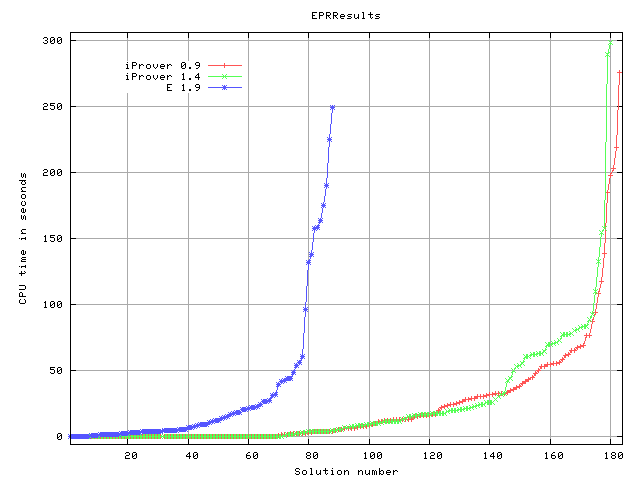
\includegraphics[scale=0.5]{pictures/EPRResults-Proof-Time.png}
		\caption{EPR division results taken from \url{http://www.cs.miami.edu/~tptp/CASC/J7/WWWFiles/ResultsPlots.html} \label{fig:epr_casc_results}}
	\end{figure}


Moreover, latest results for the sub-divisions of \ac{epr} is given in Fiqure ~\ref{fig:epr_divisions_casc_results}; where sub-figure ~\ref{fig:eps_casc_results} shows the EPS results, while sub-figure ~\ref{fig:ept_casc_results} shows the EPT results. And Table \ref{table:epr_casc_results} is a summary for the results.

\begin{figure}[H]
    \centering
    \begin{subfigure}[H]{\textwidth}
        \centering
        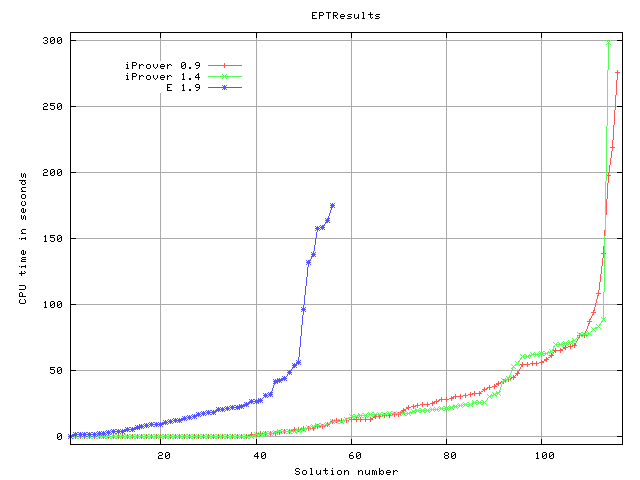
\includegraphics[scale=0.5]{pictures/EPTResults-Proof-Time.png}
        \caption{EPT sub-division results \label{fig:ept_casc_results}}
    \end{subfigure}
    ~ 
    \begin{subfigure}[H]{\textwidth}
        \centering
        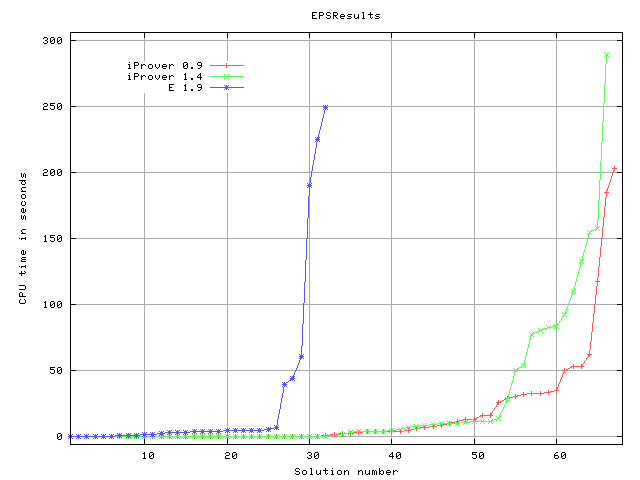
\includegraphics[scale=0.5]{pictures/EPSResults-Proof-Time.png}
        \caption{EPS sub-division results \label{fig:eps_casc_results}}
    \end{subfigure}
    \caption{EPR sub-divisions results both taken from \url{http://www.cs.miami.edu/~tptp/CASC/J7/WWWFiles/ResultsPlots.html} \label{fig:epr_divisions_casc_results}}
\end{figure}


\begin{table}[H]
	\centering
	\begin{tabular}{||c | c | c | c||} 
 		\hline
		criteria & iProver-0.9 & iProver-1.4 & E-1.9 \\ %[0.5ex] 
 		\hline\hline
		Solved(200) & 183 & 180 & 88 \\
		Average-CPU-time & 22.96 & 22.80 & 31.02 \\
		Solutions & 62 & 174 & 88 \\
		New-Solved(10) & 10 & 9 & 5 \\ [1ex] 
 		\hline
		\end{tabular}
	\caption{Summary for EPR division results}
	\label{table:epr_casc_results}
\end{table}

%TODO :: say that it will appear later



\section{\ac{epr} reasoning Techniques}
Reasoning in \ac{epr} is very interesting, since it is a fragment of \ac{fol} that could be transformed to propositional logic with some processing such as grounding techniques. So both reasoning techniques done for \ac{fol} and propositional logic are valid for \ac{epr} fragment, however for the propositional case further handling will be required.


According to \cite{EPR_PHD}, we could classify some of the methods used in reasoning for \ac{epr} fragment into two categories:
	\begin{itemize}
		\item Grounding based methods, which are mainly techniques applied to limit the number of generated clauses in the grounding step, afterwards normal methods of reasoning for propositional calculus could be applied as the \ac{epr} problem will be reduced to a propositional one. Some of those grounding based methods are mentioned below: 
			\begin{itemize}
				\item Splitting
				\item Pure Predicates
				\item Linking restrictions
				\item Sort inference
				\item Incremental Search			
			\end{itemize}
		\item Non-grounding based methods, which are methods using normal inference systems and calculi used for generic \ac{fol}.
			\begin{itemize}
				\item Resolution Calculus, which was first proposed in \cite{RES_65}
				\item Model evolution Calculus, which was proposed by \cite{MOD03}  
				\item Instantiation Calculus, which was proposed in \cite{INST03}
			\end{itemize} 
	\end{itemize}		

Resolution is the oldest one of all the three calculi. In the beginning the results mentioned in \cite{RES76} showed that it is difficult to be able to decide \ac{epr} fragment using a resolution procedure. Later on, a resolution procedure was found to be able to decide \ac{epr} \cite{RES93}. However, resolution is inefficient at least practically for \ac{epr} and this could viewed from the results of the \ac{epr} division in the yearly CASC competition.   	   


Model evolution calculus has the same decidability for \ac{fol} as resolution with saturation as proposed here in \cite{BAGA01}. So it is refutationally complete and sound. But it has an advantage over resolution, since it is in general a decision procedure for \ac{epr} fragment, however this is not the case with most resolution procedures. And practically the automated theorem provers that implement the Model evolution calculus have better results in the CASC competition for \ac{epr} division.


Instantiation Calculus has the same decidability for \ac{fol} as resolution with saturation and model evolution calculus. And it is decision procedure for \ac{epr} fragment like Model evolution calculus. And the automated theorem provers that depends on Instantiation calculus have a very good results in the CASC competition for the \ac{epr} division \cite{CASC_24,CASC_J7}, at least the first on this division in the last CASC competition. CASC-J7. is an Instantiation based theorem prover.

 
Table \ref{table:cal_comp} found below summarizes the comparison between the three Non-grounding methods for reasoning in \ac{epr}.

	\begin{table}[H]
		\centering
		\begin{tabular}{||c | c | c | c||} 
 			\hline
			Point of Comparison & Resolution & Model Evolution & Instantiation \\ %[0.5ex] 
 			\hline\hline
			Relatively New & No & Yes & Yes \\
			Semi-decidable for \ac{fol} & Yes & Yes & Yes \\
			Decidable for \ac{epr} & No, in general & Yes & Yes \\
			Practically proved efficiency in \ac{epr} division & No & Yes & Yes \\ 
			Example for Prover	& E	& Darwin		& iProver \\ [1ex] 
 			\hline
		\end{tabular}
		\caption{Summary for Non-grounding methods for reasoning in \ac{epr}}
		\label{table:cal_comp}
	\end{table}



\section{Range Restricting Transformations}
According to \cite{BMUG06}, The range restricted transformations implemented in this project, that was originally devised in \cite{BMUG06}, were also added to other theorem provers MSPASS and KRHyper. And the results showed improvement and effectiveness in trying them over the satisfiable set problems in TPTP, specifically Version 3.1.1.   
